\vspace{-.5cm}
\section{The Running Example: Quiz Controller}
\label{sec:example}
\vspace{-.3cm}
Our running example for this demonstration is a controller for a system that
allows playing quiz games -- quiz controller (QC) for short. The controller
blinks indicator light for the assigned user (i.e., pupil, professor and high
school in our running example) and enables the user to answer the quiz
questions.
We directly illustrate the behavior of the controller that we are building as a
set of \textsf{EARS-CTRL} requirements as shown in figure~\ref{fig:QC_reqs}. Given the requirements are written in English, they are self-explanatory.
\begin{figure*}[!h]
\centering
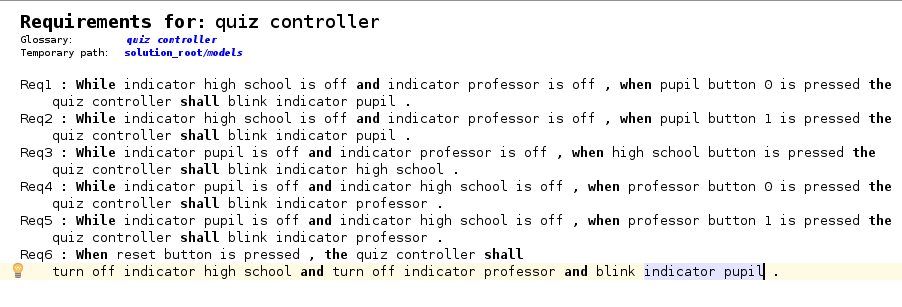
\includegraphics[width=1\textwidth]{./images/QC_Reqs.png}
\caption{Requirements written in \emph{EARS-CTRL} for a Quiz Controller}
\label{fig:QC_reqs}
\end{figure*}
